%%%%%%%%%%%%%%%%%%%%%%%%%%%%%%%%%%%%%%%%%%%%%%%%%%%%%%%%%%%%
\subsection{Sensitivity of NEXT-100}
%%%
The sensitivity of NEXT-100 to neutrinoless double beta decay --- calculated following the Feldman-Cousins prescription for the construction of confidence intervals \cite{Feldman:1997qc, GomezCadenas:2010gs} --- is shown in Figure~\ref{fig:SensitivityNEXT100}. In the top panel, the sensitivity (at 90\% CL) to the half-life (red, solid curve) and the corresponding sensitivity to \mbb\ (blue, dashed curves) for the largest and smallest nuclear matrix element calculations published (e.g, the ISM model predicts an NME of 2.19 \cite{Menendez:2008jp} 
while  \cite{Yao:2014uta} finds a value of 4.32 using the EDF model). 
are represented in terms of the exposure, assuming a signal detection efficiency of 28\% and a background rate of $6\times10^{-4}~\ckky$. The bottom panel shows, for an exposure of 100~kg$\cdot$year the variation of the sensitivity with respect to the background rate in the range between $10^{-5}$ and $10^{-4}$~\ckky.


%%%%%%%%%%
\begin{figure}
\centering
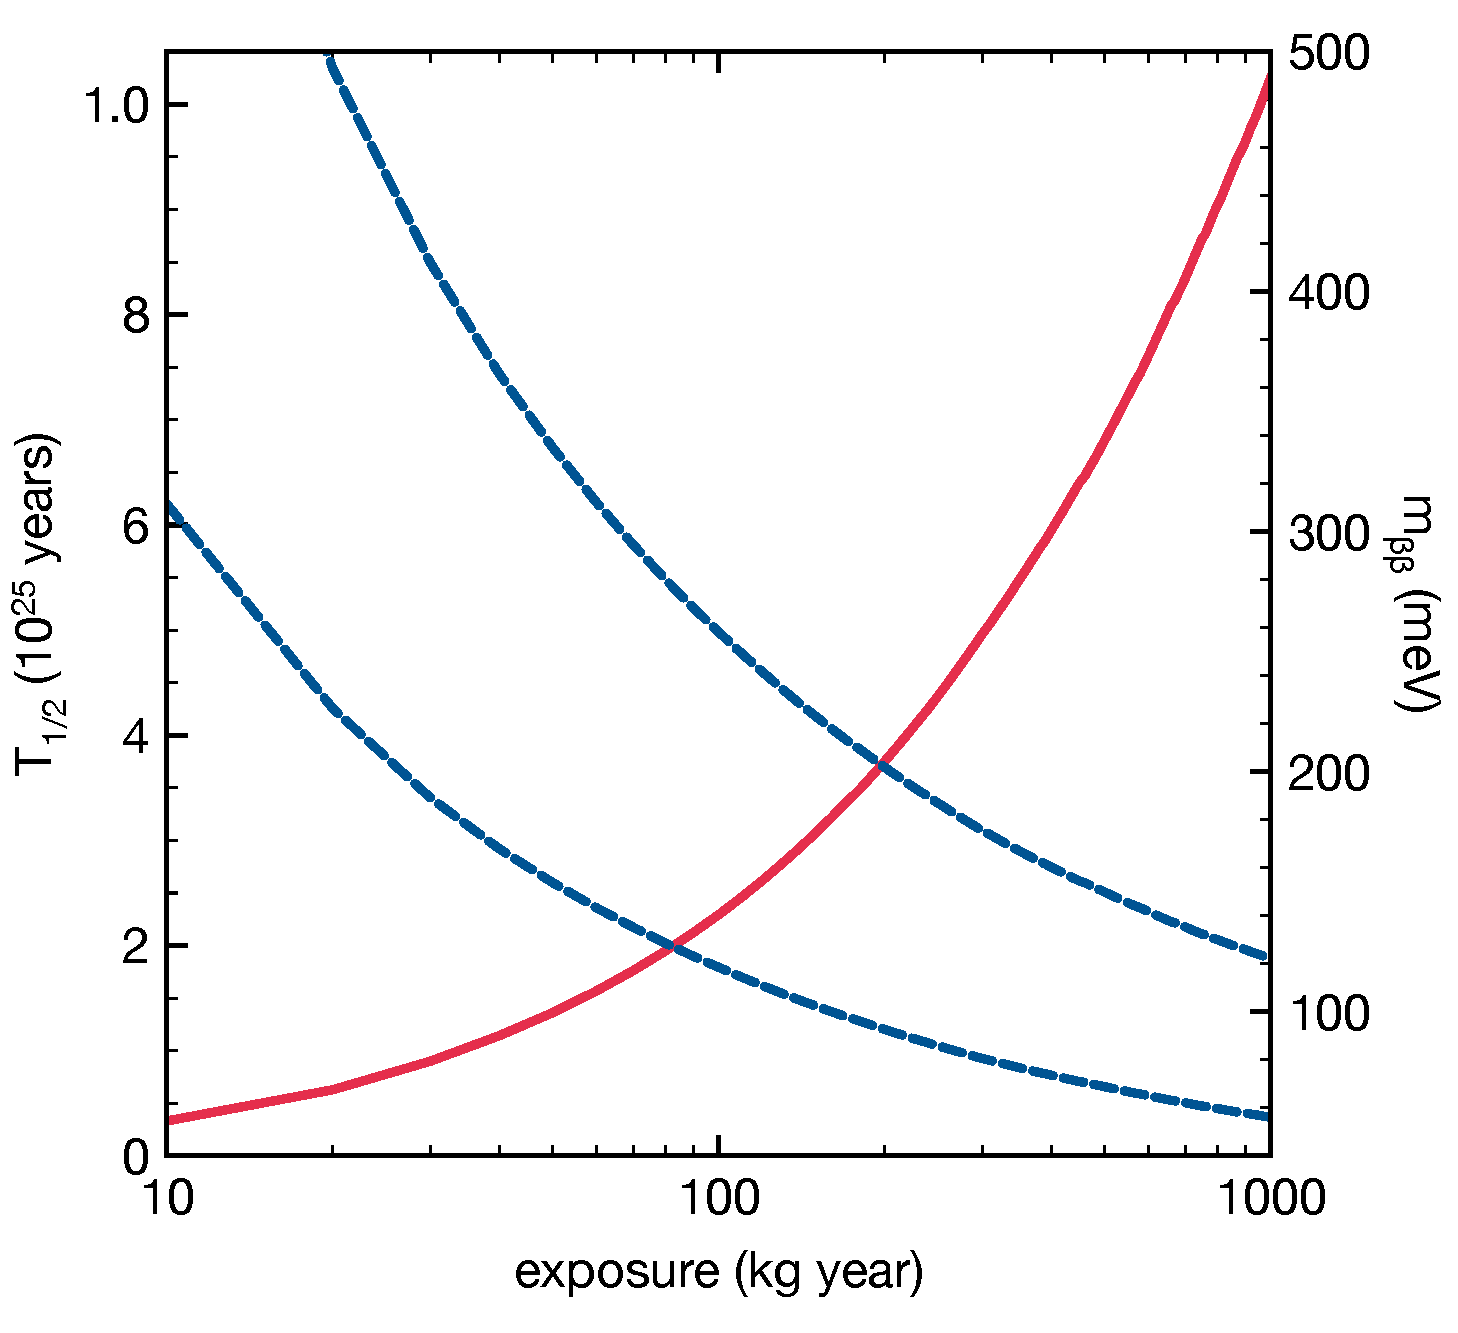
\includegraphics[width=0.7\textwidth]{img2/Next100SensitivityVsExposure.pdf}
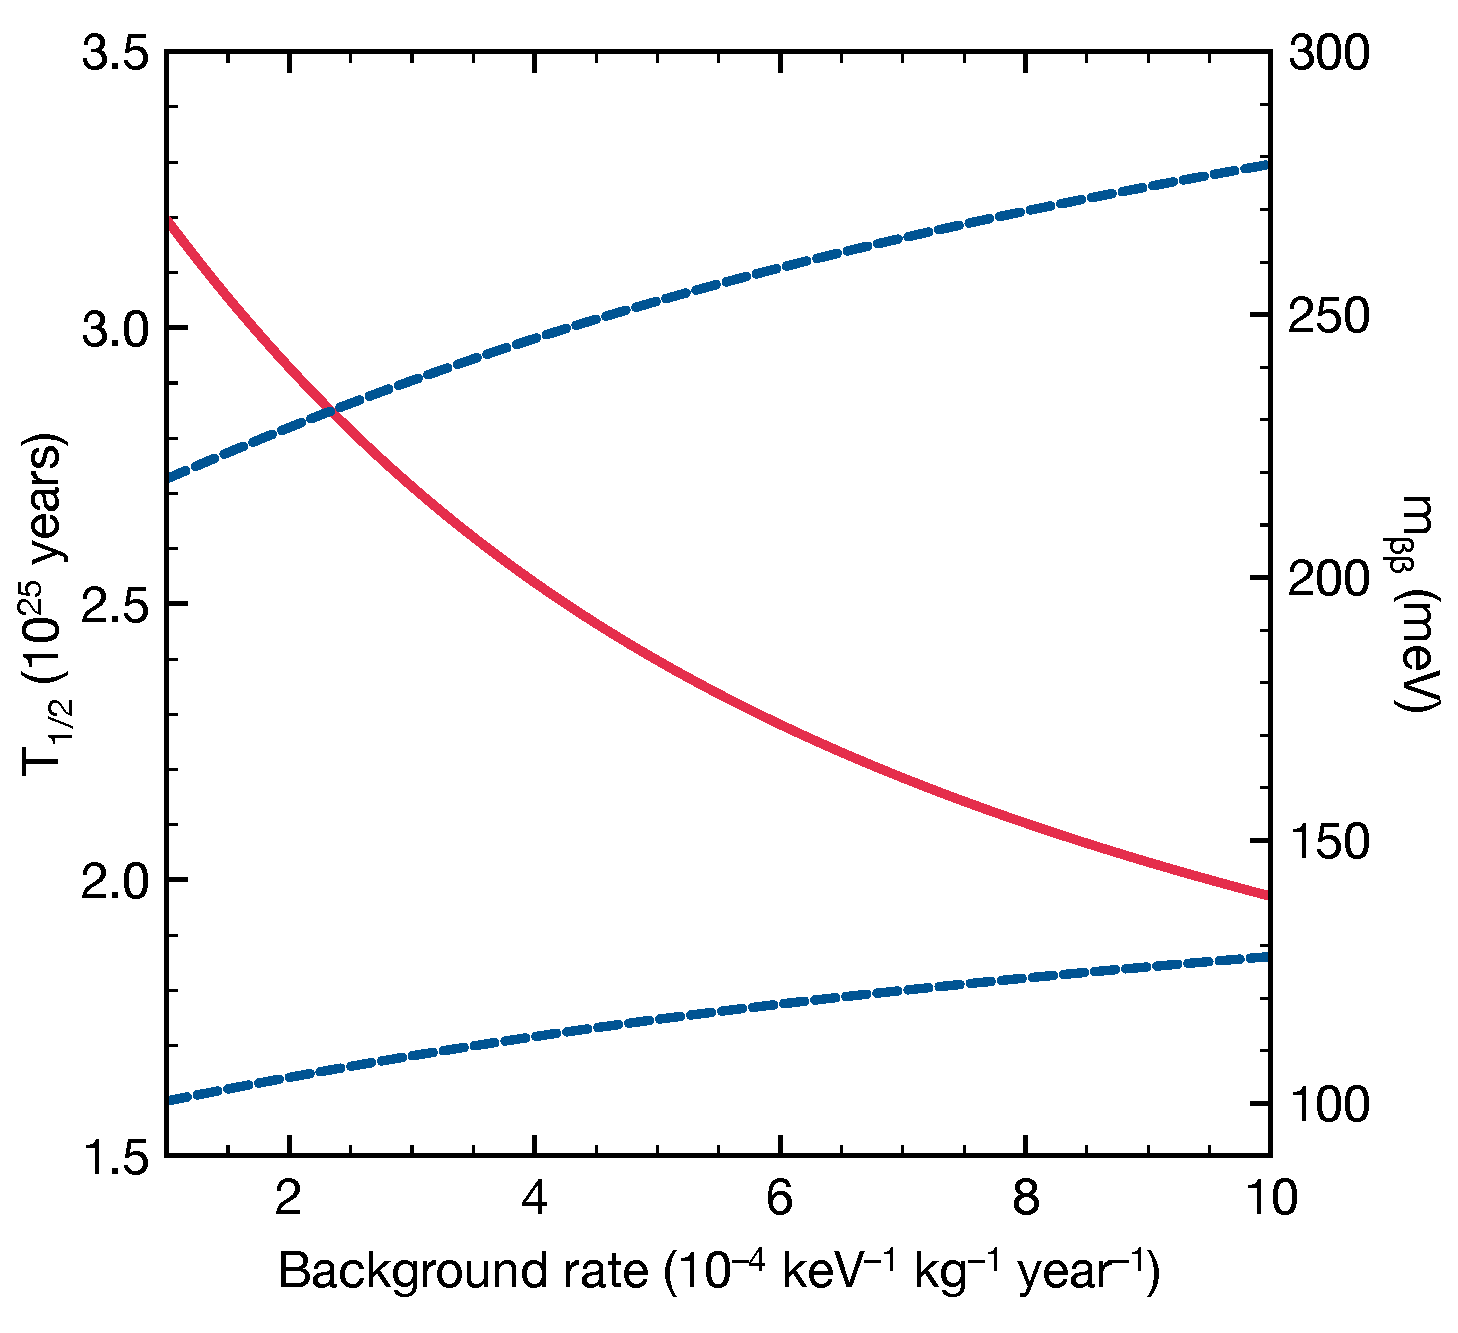
\includegraphics[width=0.7\textwidth]{img2/Next100SensitivityVsBackground.pdf}
\caption{Sensitivity of NEXT-100 to neutrinoless double beta decay. Top: Sensitivity (at 90\% CL) to the \bbonu-decay half-life (red. solid curve) and the corresponding \mbb\ sensitivity (blue, dashed curves) for the largest and smallest NME calculations in terms of the exposure. Bottom: Sensitivity (at 90\% CL) in terms of the background rate.} \label{fig:SensitivityNEXT100}
\end{figure}
%%%%%%%%%%
